\documentclass[a4paper,11pt,twoside]{article}
\usepackage[swedish]{babel}
\usepackage[T1]{fontenc}
\usepackage[utf8]{inputenc}
\usepackage{lmodern}
\usepackage{verbatim}
\usepackage{multicol}
\usepackage{hyperref}
\usepackage{listings}
\usepackage{color,hyperref}
\usepackage{csquotes}
\usepackage{fancyhdr}
\usepackage{courier}
\usepackage{color}
\usepackage{amsmath}
\usepackage{graphicx}
\usepackage{bbm}
\usepackage{amssymb}
\usepackage{wrapfig}
\usepackage{float}
\newcommand*\colvec[3][]{
    \begin{pmatrix}\ifx\relax#1\relax\else#1\\\fi#2\\#3\end{pmatrix}
}
\usepackage[numbered,framed]{matlab-prettifier}
\newfloat{listing}{H}{lst}%[section]
\title{Pilbåge}
\author{
  Viktor Kronvall 920225-5478 \\
  Christopher Lillthors 911005-3817 \\
  \\
  Numeriska metoder SF1541
}
\pagestyle{fancy}
\setlength{\headheight}{54pt}
\fancyfoot[C]{}
\fancyfoot[RO, LE] {\thepage}
\lhead{\textbf{Kungliga Tekniska Högskolan} \\ Civilingenjör datateknik\\ Numeriska metoder SF1541}
\rhead{\textbf{Pilbåge} \\ \date{\today} \\ \ \\}
\setlength{\parindent}{0in}
\setlength{\parskip}{0.1in}
\date{\today}

\lstMakeShortInline"
\lstset{
  style              = Matlab-editor,
  basicstyle         = \mlttfamily,
  escapechar         = ",
  mlshowsectionrules = true,
}

\begin{document}
\maketitle
% for the lulz...
\begin{frame}
\null
\vfill
Generated in \LaTeX
\end{frame}
\thispagestyle{empty}
\newpage
\tableofcontents
% \lstlistoflistings
\thispagestyle{empty}
\newpage
\clearpage
\setcounter{page}{1}
%	Actual document begins here...
\section{Problem}
Det problem som löses i denna rapport är att bestämma vilken form en pilbåge skapad av en linjal och ett snöre får givet en differentialekvation och den kraft som verkar i bågsträngen.

Formen på pilbågen är symmetrisk och defineras av följande ekvation:
\begin{equation} \label{eq:original}
	\dfrac{d^2y}{dx^2} + qy + \left(1+\left(\dfrac{dy}{dx}\right)^2\right)^{3/2} = 0
\end{equation}

och dessa givna randvilkor: $y(0)=0.3,\: y'(0)=0,\: y(a)=0$ där pilbågen är definerad i punkterna $x \in [-a,a]$.

Pilbågens båglängd mellan $x=0$ och $x=a$ är dessutom definerad till att vara $0.5$m lång. Där båglängden $s$ beskrivs av ekvationen:
\begin{equation}
s = \int_0^a{\sqrt{1+y'(x)^2}}=0.5 \nonumber
\end{equation}
\begin{figure}[h!]
\caption{Illustration av pilbågen}
\centering
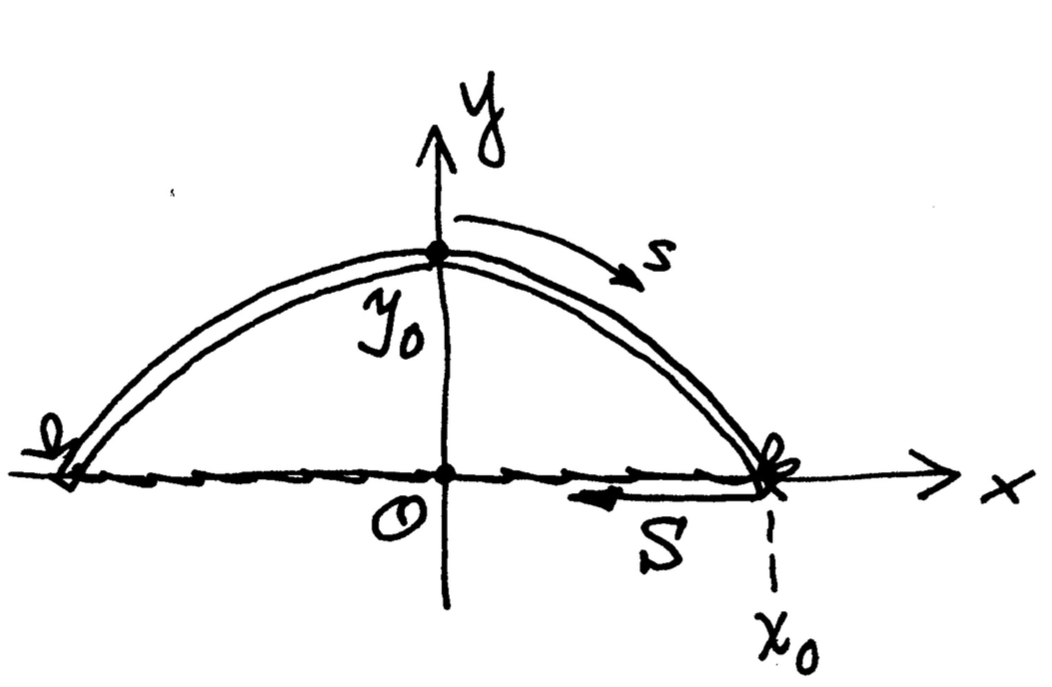
\includegraphics[scale=0.3]{bild.png}
\end{figure}
\newpage
\section{Lösning}
\subsection{Startvärden}
Eftersom att $q$ är okänd så blir då ekvation ~\eqref{eq:original} ganska komplicerad att lösa och därför försöker vi först hitta ett ungefärligt värde till $q$ genom att förenkla ekvationen till:
\begin{equation} \label{eq:simplified}
	\dfrac{d^2y}{dx^2} + qy = 0
\end{equation}
Detta kan vi göra eftersom derivatan $\left(\dfrac{dy}{dx}\right)^2$ är mycket liten
inom intervallet.

Denna differentialekvation löses sedan analytiskt genom att ansätta $y=e^{rx}$ där $r \in \mathbb{N}$
Detta ger den karaktäristiska ekvationen $e^{rx}(r^2+q)=0$ med röttterna $r=\pm \sqrt{q}\:i$.
Med standardlösningar erhålles därigenom följande ekvationer:
\begin{equation}
 y(x) = A cos(\sqrt{q}\:x)+B sin(\sqrt{q}\:x) \nonumber
\end{equation}
\begin{equation}
 y'(x) = -A\sqrt{q}\: sin(\sqrt{q}\:x) + B\sqrt{q}\:cos(\sqrt{q}\:x) \nonumber
\end{equation}
Insättning av begynnelsevärdena i ovanstående ekvationer ger:
\begin{equation} \label{eq:y}
 y(x) = 0.3 cos(\sqrt{q}\:x)
\end{equation}
\begin{equation} \label{eq:yprime}
 y'(x) = -0.3\sqrt{q}\: sin(\sqrt{q}\:x)
\end{equation}
Dessutom följer sambandet $a=\dfrac{\pi}{2\sqrt{q}}$ ur ekvation ~\eqref{eq:y} då pilbågen kan antas vara icke-periodisk.

Med hjälp av Matlab-rutinen \textit{ode45}, som använder sig av fjärde och femte ordningens Runge-Kuttametoder, löses ekvationerna ~\eqref{eq:y} och ~\eqref{eq:yprime} och båglängden för ett givet $q$ kan bestämmas.

Sekantmetoden används sedan för att finna det $q$ som motsvarar en båglängd på en halv meter. Det vill säga, en rot till f(s) = s-0.5 finnes.

\subsection{Lösning av ursprungliga ekvationen}
När ett approximativt $q$ väl har funnits med hjälp av ekvation ~\eqref{eq:simplified} kan detta användas som startvärde till lösning av ekvation ~\eqref{eq:original}.

Sekantmetoden används återigen för att lösa differentialekvationen. Denna gång behöver ekvationen dock skrivas om som flera differentialekvationer av första ordningen där $x$ är en fri variabel.
\begin{align}
\begin{tabular}{ l l }
	$u_1 = y$ & $u_1' = u_2$ \\
	$u_2 = y'$ & $u_2' = -qu_1\left(1 + \left(u_2\right)^2\right)^{3/2}$
\end{tabular}
\nonumber
\end{align}

Nu löses återigen systemet med \textit{ode45}. Punkten $x=a$ finnes genom  kriteriet då y-värdet passerar x-axeln.

Koden för detta kriterie är som följande:
\begin{listing}
\lstinputlisting[caption = {findroot.m}]{../labb3/findroot.m}
\lstinputlisting[caption = {ursprunglig.m}]{../Labb3/ursprunglig.m}
\end{listing}

Följaktligen löses systemet återigen med sekantmetoden och det $q$ som ger en båglängd på en halv meter väljs.

Den kraft som verkar i bågsträngen bestäms med hjälp av momentet i en punkt $M(x)$ som beskrivs enligt:
\begin{equation}\label{eq:moment}
M(x) = -qy(x)
\end{equation}
Ytterligare gäller att momentet
\begin{equation}
	S \times r = M(x)
\end{equation}
där $r$ är momentarmen och $S$ är den kraft som verkar ortogonalt mot momentarmen $r$. Momentarmen $r$ defineras som:
\begin{equation}
	r(x) = \colvec{a}{0}-\colvec{x}{y(x)}
\end{equation}
Eftersom kraften går längs linan (som i sin tur är längs x-axeln), blir det ortogonala komplementet endast längs y-axeln och därför blir den ortogonala komponenten av $r(x) = -y(x)$.

Detta ger $\forall x, S = q$.

\subsection{Utvidning och lösning med s som fri variabel}
Ovanstående problem kan även lösas med $s$ som fri variabel istället för $x$. I detta fall observerar vi att krökningen i pilbågen är $-qy$. Då beskrivs lösningen istället av följande differentialekvation:
\begin{equation}
	\dfrac{d^2y}{ds^2}+qy\left(\dfrac{dx}{ds}\right)=0, \quad \dfrac{dx}{ds} = \sqrt{1-\left(\dfrac{dy}{ds}\right)^2}
\end{equation}

Differentialen löses med \textit{ode45} och ett ekvationssystem med tre första ordningens differentialekvationer:

\begin{align}
\begin{tabular}{ l l }
	$u_1 = x$ 					& $u_1' = \sqrt{1-(u_3)^2}$\\
	& \\
	$u_2 = y$ 					& $u_2' = u_3$\\
	& \\
	$u_3 = \dfrac{dy}{ds}$ 		& $u_3' = -qu_2\sqrt{1-(u_3)^2}$
\end{tabular}
\nonumber
\end{align}

Eftersom $s$ är avståndet från punkten $\colvec{0}{0.3}$ längs pilbågen finner vi att $x(s)=0, y(s)=0.3$ då $s=0$. Derivatan i startpunkten $\dfrac{dy}{ds}(0)$ finnes genom förhållandet:
\begin{equation}
\dfrac{dy}{ds}=\dfrac{dy}{dx}\cdotp\dfrac{dx}{ds} \nonumber
\end{equation}
Givet det ursprungliga randvillkoret $\dfrac{dy}{dx}=0$ då $x=0$ och det att $x=0$ då $s=0$ finner vi att $\dfrac{dy}{ds}=0$ då $s=0$.

Detta ger begynnelsevillkoren:
\begin{equation}
\colvec[x]{y}{\dfrac{dy}{ds}}=\colvec[0]{0.3}{0} \nonumber
\end{equation}

Differentialekvationen löses med $s \in [0,0.5]$ för ett givet $q$ och det $q$ som resulterar i att ändpunktens y-värde är lika med $0$ finnes med sekantmetoden.

\section{Implementation}
\href{https://github.com/christopherL91/Numme14}{https://github.com/christopherL91/Numme14}
\end{document}